\section{Une approche dédiée au domaine de l'assistance domiciliaire}
Nous présentons ici les étapes principales de notre approche spécifique au domaine 
pour développer des services sensibles au contexte dédié au maintien à domicile 
des personnes âgées.

La fourniture d'un service sensible au contexte, selon notre approche, implique deux phases principales, illustrées en Figure~\ref{fig:functionalarchi}: 
\begin{itemize}
\item La phase de développement~: les intervenants définissent un service sous 
forme de règle en langage Maloya. Cette règle métier est ensuite compilée vers une règle de plus bas niveau en 
langage de traitement d'évènements. Les outils assistant le développeur de service lors de cette phase comprennent le 
compilateur et une interface de gestion des services.
\item La phase d'exploitation~: les services compilés sont exécutés sur les flux 
d'évènements provenant d'une maison sensible au contexte. Une fois mise en place, une règle est 
exécutée de façon à révéler chaque occurrence de la séquence d'évènements 
qu'elle décrit, jusqu'à ce que la règle soit supprimée, ou mise à jour. 
La phase d'exploitation est implantée par un analyseur d'évènements d'interaction qui 
transforme ces évènements en une forme canonique appelée {\em StreamEvent} 
(ou simplement, flux d'évènement, par la suite) pour alimenter un moteur de traitement d'évènements 
complexes (CEP). Ce moteur CEP est chargé de l'exécution des règles compilées sur le flux d'évènements.
%qui exécute les règles sur ce flux d'èvenements et retourner un signal lorsqu'une séquence d'évènements correspondant à une règle est identifiée dans le flux. 
\end{itemize}
\begin{figure*}[h]
\centering
  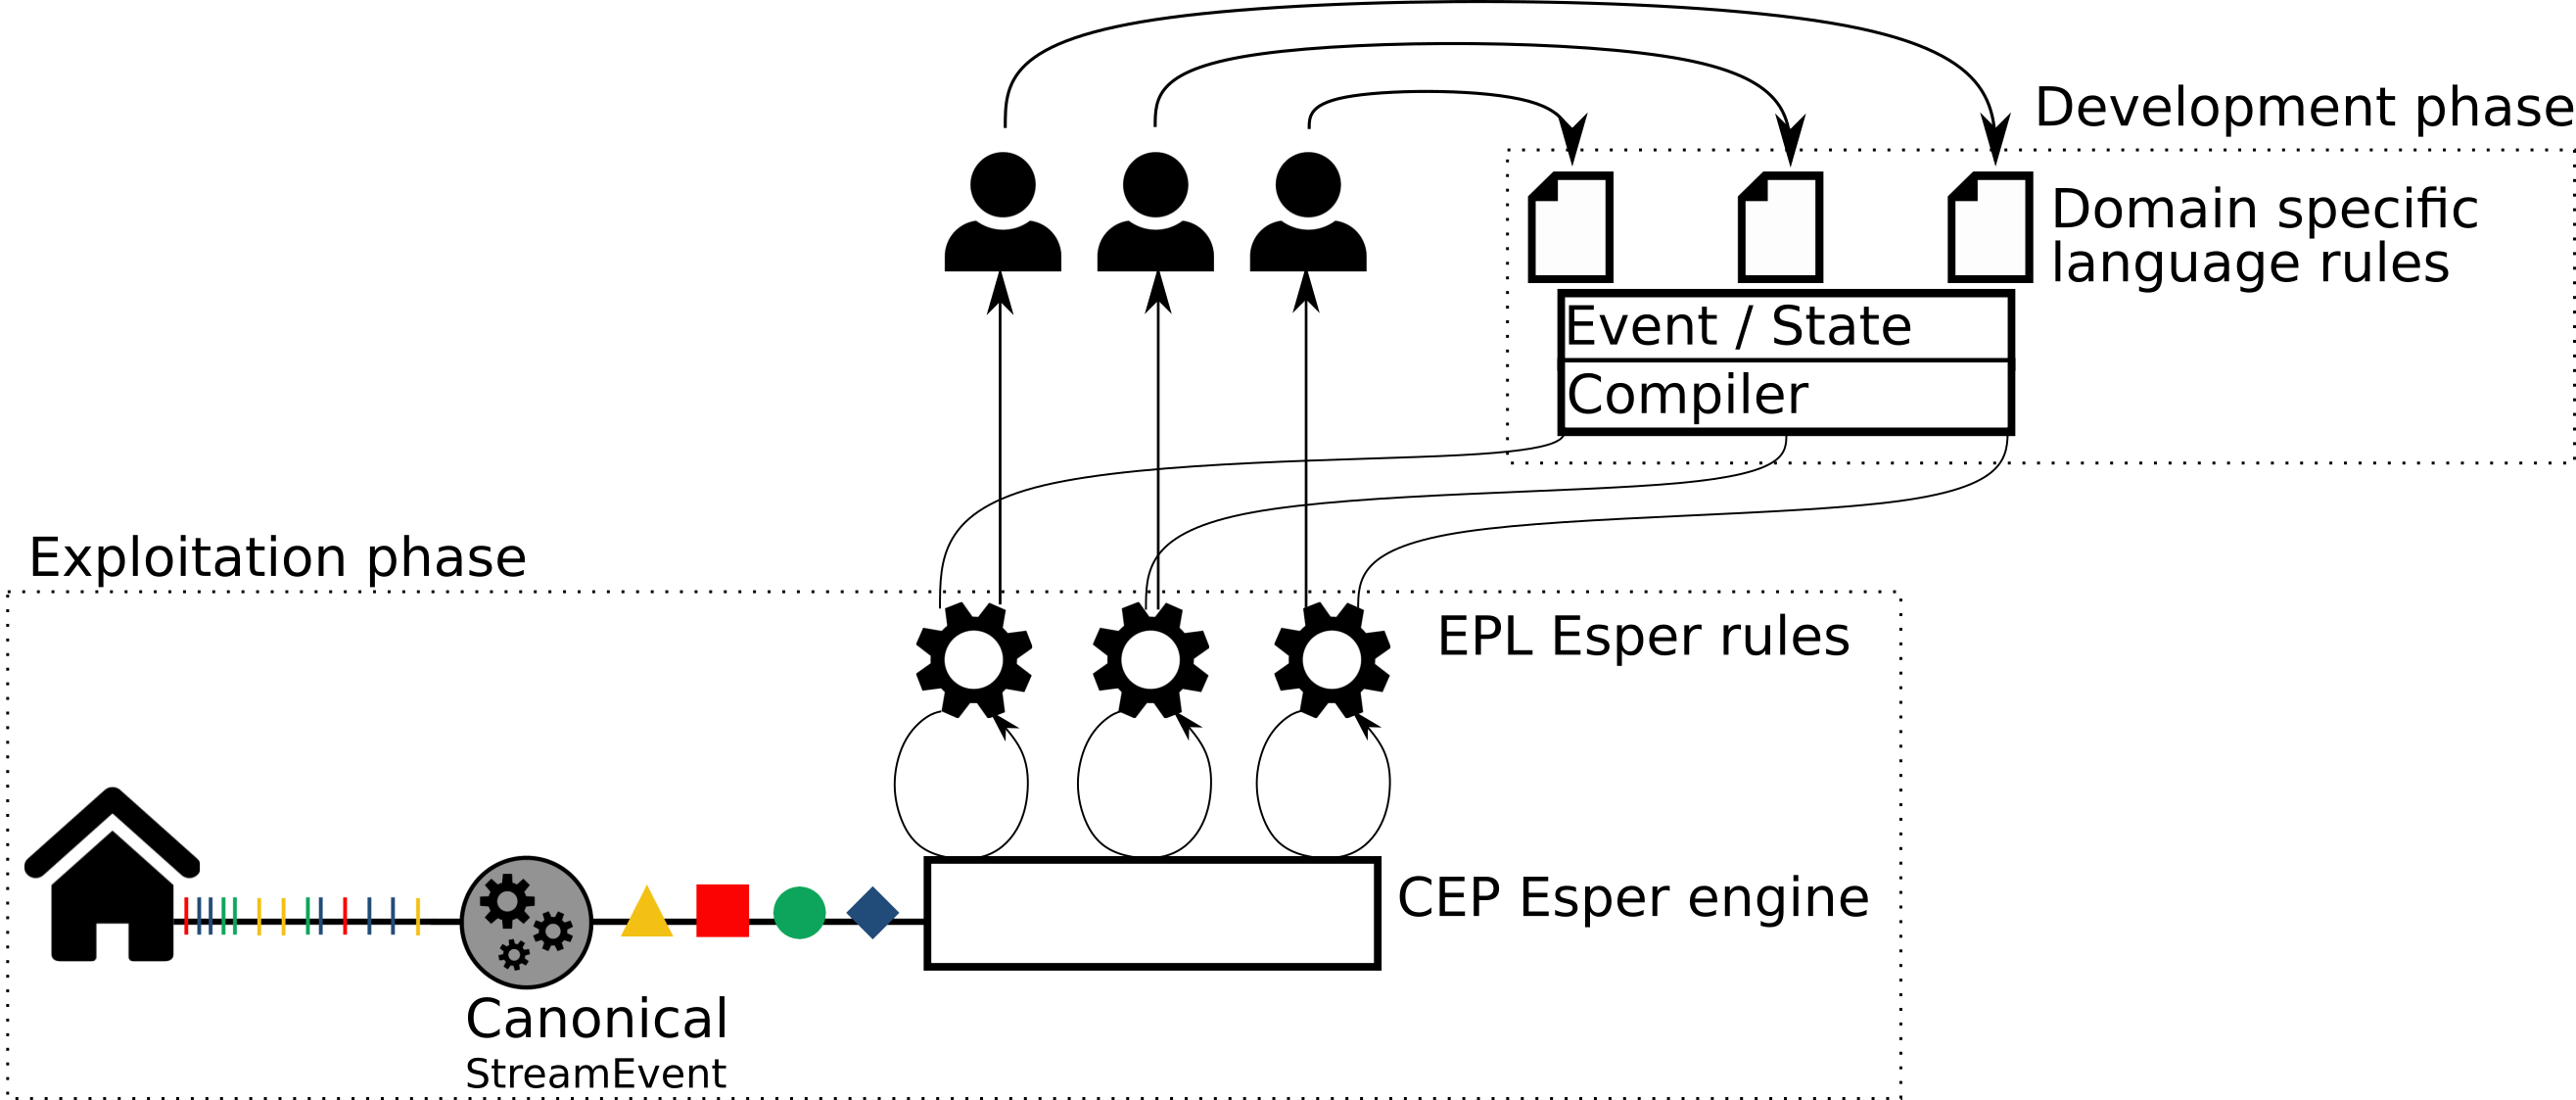
\includegraphics[width=\linewidth,totalheight=\textheight,keepaspectratio]{gfx/approach}
\caption{Vue globale de notre approche dédiée au domaine.}
\label{fig:functionalarchi}
\end{figure*}

\subsection{Définition du service}
La première étape est initiée par les intervenants qui expriment les scénarios 
de services. Ces scénarios sont soit directement écrits dans notre langage dédié par 
l'intervenant en exploitant les concepts d'états/évènements et les opérateurs 
de composition disponibles, si ils ont le bagage nécessaire, soit par un 
développeur de services, dans le cas contraire.
% dans le langage coeur

Notre implantation offre une interface graphique simple pour définir, compiler,
supprimer, et mettre à jour un service, 
comme illustré en Figure~\ref{fig:ui_rule}.
\begin{figure*}[h]
\centering
  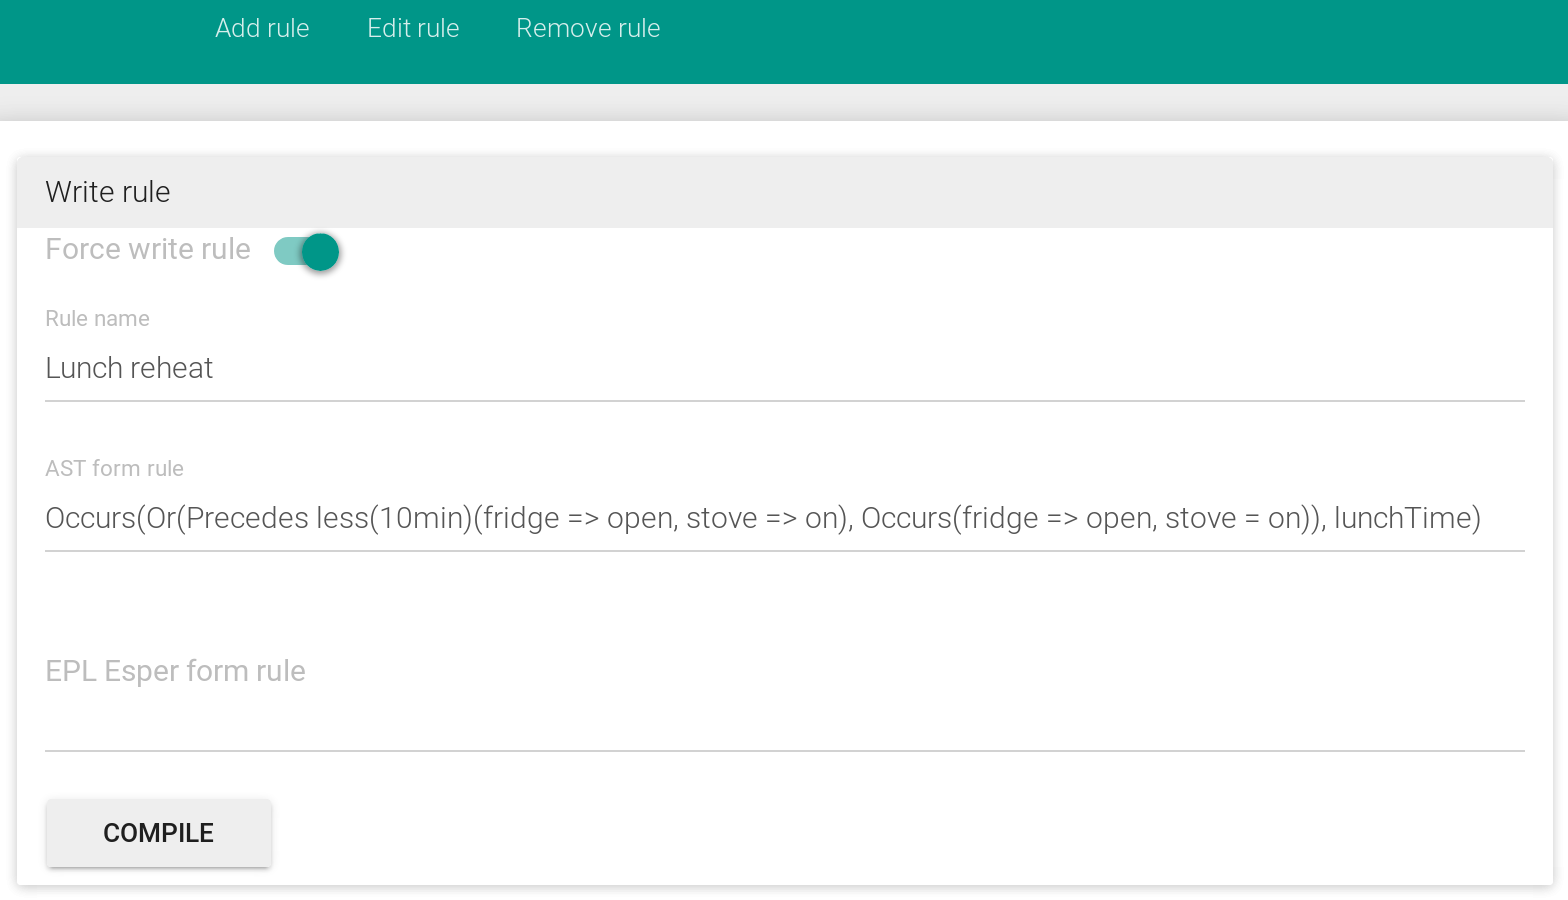
\includegraphics[width=\linewidth,totalheight=\textheight,keepaspectratio]{gfx/ui_add_rule}
\caption{Interface d'administration de service.}
\label{fig:ui_rule}
\end{figure*}

\subsection{Compilation du service}
Les services de haut niveau sont compilés vers un langage de traitement d'évènements qui exprime des règles de plus bas niveau. 
Le langage cible de traitement d'évènements ne supporte pas directement la notion d'état ainsi que nos opérateurs. Lors des étapes de compilation, ces concepts sont donc explicités sous forme de combinaisons d'évènements correspondants.

\subsection{Exécution du service}
Pour être déployées, les règles compilées sont enregistrées auprès du moteur CEP. Notre moteur d'exécution de règle est basé sur Esper, un CEP open-source développé par EsperTech\footnote{\url{http://www.espertech.com/esper/}}. 
Esper propose des interfaces Java et .Net avec NEsper, en tant que bibliothèques pour développer des programmes 
événementiels. Nous avons choisi Esper parce qu'il s'agit d'un moteur CEP 
populaire utilisé à la fois dans l'industrie et dans la recherche. Esper fournit 
un langage spécifique et déclaratif pour le traitement d'évènements complexes, 
appelé EPL (pour Event Processing Language). 
Ce langage inclut tous les opérateurs de SQL, et ajoute des constructions telles que la définition et l'interaction avec des fenêtres, ainsi que pour la génération de sorties.
EPL permet également de décrire des motifs 
d'évènements (ou ``Patterns'' EPL) à identifier dans un flux d'évènements temps réel, en utilisant des 
opérateurs pour ordonner les évènements, des contraintes temporelles, {\em etc.}. Ces opérateurs peuvent s'imbriquer
et permettent de définir explicitement la politique de sélection d'évènements avec la clause ``every''. 
Esper permet de recevoir les données en sorties d'une règle, soit en mode push, par l'utilisation de listeners, soit en mode pull, en utilisant des itérateurs.
%La seconde manière d'exprimer les motifs d'évènements utilise des expressions régulières. 
%Les deux syntaxes offrent la même expressivité.
% Esper propose des interface Java et C\# pour développer des programmes 
% événementiels. Nous avons choisi Esper parce qu'il s'agit d'un moteur CEP 
% populaire utilisé à la fois dans l'industrie et dans la recherche. Esper fournie 
% un langage spécifique et déclaratif pour le traitement d'évènements complexes, 
% appelé EPL (pour Event Processing Language). EPL permet de décrire des motifs 
% d'évènements à identifier dans un flux d'évènements temps réel, en utilisant des 
% opérateurs pour ordonner les évènements, des contraintes temporelles, {\em etc.} 
Cependant, Esper ne permet pas de manipuler le concept d'état, d'où la nécessité
d'encoder cette notion par des motifs purement évènementiels. 

\subsection{Forme canonique}
La forme canonique des données produites par un domicile sensible au contexte 
permet de traiter les mesures d'interaction indépendamment 
de leur format original. Cette forme canonique 
de données, nommée {\em StreamEvent}, est ainsi une couche d'abstraction sur l'hétérogénéité
des évènements des différentes sources, constituant un flux d'évènements uniforme. 
Dans cette représentation, chaque évènement est un 
quadruplet comprenant le type de l'évènement, sa localisation, sa valeur, et l'horodatage de son occurrence.

\[K\] (pour Kinds) est l'ensemble des types d'interactions (\eg Freezer)
\[L\] (pour Locations) est l'ensemble des localisation d'interactions (\eg Kitchen)
\[V\] (pour Values) est l'ensembles des valeurs de chaque domaine d'interaction (\eg open/close)
\[\mathds{N}\] est l'ensemble des horodatages (timestamps) d'instances d'interactions
\[
  v \in \mathds{V} \in \overset{m}{\underset{j=0}\cup}D_{K_i}
\] 
\[ 
t \in \mathds{N}
\]
in
\[
  s \in S=\mathcal{P}(K\times L\times \mathds{V}\times \mathds{N})
\]
\[
  s =\{(k_0,l_0,v^{D_{k_0}}_0,t_0), \dots, (k_n,l_o,v^{D_{k_n}}_n,t_n)\}
\]

Notons que le flux d'évènements en format StreamEvent ainsi défini est plus bas niveau que
le format des rôle défini en Section~\ref{archi:algebra}. En effet, comme dans les langages de CEP, utilisés comme cible,
les évènements sont toujours ponctuels (\ie n'ont pas de durée)\footnote{Même
dans les langages CEP avec une sémantique d'intervalle, les évènements élémentaires
sont toujours ponctuels, comme discuté en Section~\ref{sec:cep}.}, nous ne pouvons pas réutiliser
directement les évènements de rôles, qui étaient estampillés par des intervalles de temps (les périodes).
En revanche, ce nouveau format permet de détecter de manière plus précoce certains évènements
complexes, sans attendre la fin d'un évènement, pouvant avoir une durée non négligeable. Par exemple,
prenons la règle vérifiant si une porte reste ouverte pendant plus de 3 heures. Avec un log
d'évènements de rôles, cette règle ne pouvait déclencher que lorsque la porte était refermée,
car c'est à ce moment-là que l'évènement ``interaction de porte'' se produisait. Au contraire,
avec un log en format StreamEvent, il devient possible d'observer l'ouverture de porte indépendamment
de sa fermeture, et donc de réagir, en principe, dès que le délai de 3 heures s'est écoulé. Nous
verrons par la suite comment notre langage dédié atteint effectivement cette réactivité en
s'appuyant sur le langage cible Esper. Ce niveau de réactivité n'était pas capital dans le contexte
du Chapitre~\ref{cha:fiabilite}, où le signalement à la volée des dysfonctionnements des capteurs 
servait au service de maintenance, ayant un cycle d'intervention de l'ordre de plusieurs jours. Il en
est tout autrement dans le contexte du chapitre actuel où l'on s'intéresse à une classe bien plus large de services,
incluant des assistances de sécurité et des rappels d'activités.
